% Author: David Larsen <dcl9934@cs.rit.edu>
\documentclass[11pt]{article}
\usepackage{fullpage}
\usepackage{listings}
\usepackage{needspace}
\usepackage{color}
\usepackage{ifthen}
\usepackage{pgf}
\usepackage{tikz}
\usetikzlibrary{arrows,automata}
\usepackage{csc}

\lstset{ %
basicstyle=\footnotesize,       % the size of the fonts that are used for the code
numbers=left,                   % where to put the line-numbers
stepnumber=1,                   % the step between two line-numbers. If it's 1 each line will be numbered
numbersep=5pt,                  % how far the line-numbers are from the code
showspaces=false,               % show spaces adding particular underscores
showstringspaces=false,         % underline spaces within strings
tabsize=4,		                % sets default tabsize to 4 spaces
language=Python
}

\ifthenelse{\isundefined{\isAnswerKey}}
{
    \newenvironment{answer}{\large\lstset{basicstyle=\large}\color{white}}{}
}
{
    \newenvironment{answer}{\large\lstset{basicstyle=\large}\color{red}}{}
}

\author{Computer Science Community}
\title{CS-242 Midterm Exam Review}
\date{Spring, 2011-3}

\makeatletter
\let\thetitle\@title
\let\theauthor\@author
\let\thedate\@date
\makeatother

\begin{document}
\header

\begin{enumerate}
\section*{Stacks and Queues}
    \item What data structure is important for doing a depth-first traversal?

        \begin{answer}
        A stack.
        \end{answer}

    \item When traversing trees last quarter, we didn't need to use either a
        stack or a queue. Why not?

        \begin{answer}
        We did depth-first traversals last quarter, when we did the pre, in and
        post-order tree traversals. We didn't need to maintain our own stack
        because our solutions were recursive: Python took care of maintaining
        the data at various stages of the traversal. Calling a function was
        like push()ing onto the stack and returning from a function was like
        pop()ing from the stack.
        \end{answer}

    \item If we wanted to implement a stack as a linked list, what linked-list
        operations would correspond to push() and pop()?

        \begin{answer}
        push( stack, element ) $\rightarrow$ insertFront( linked-list, element )\\
        pop( stack ) $\rightarrow$ removeFront( linked-list )
        \end{answer}
        
    \item Write your own stack class using python's built in lists to manage the elements of your stack. \\
    Your stack must provide the following functionality:
          \begin{itemize}
          \item []push( elm ) - push elm onto the top of the stack
          \item []pop() - return the top elm of the stack and remove it from the stack
          \item []isEmpty() - is the stack empty()
          \item []peek() - which returns the top element of the stack without modifying the stack. 
          \item []\_\_str\_\_
          \end{itemize}
          \begin{answer}
          \begin{lstlisting}
          class Stack:
            def __init__(self):
                self.lst = []
            def push(self, val ):
                self.lst.append( val )
            def pop(self):
                return self.lst.pop()
            def peek(self):
                return self.lst[-1]
            def isEmpty(self):
                return (len(self.lst) == 0)
            def __str__(self):
                return str(self.lst)
                  \end{lstlisting}
          \end{answer}

\section*{Graph Searching}
    \item If you want to find the shortest path to a node on a graph, what type
        of traversal would be best to use? Why?

        \begin{answer}
        A breadth-first traversal will {\em always} find a path with the
        minimum number of hops. This happens because we evaluate all of the
        nodes at the same distance away from the start point at the same time.
        We can say that the first time we see the node we want, we will have
        taken the shortest path to reach it.
        \end{answer}

    \item Show the principal data structure (stack or queue) for traversing the
        following graph and show the final path. When given the option to
        traverse multiple nodes, go in alphabetical order.
     
           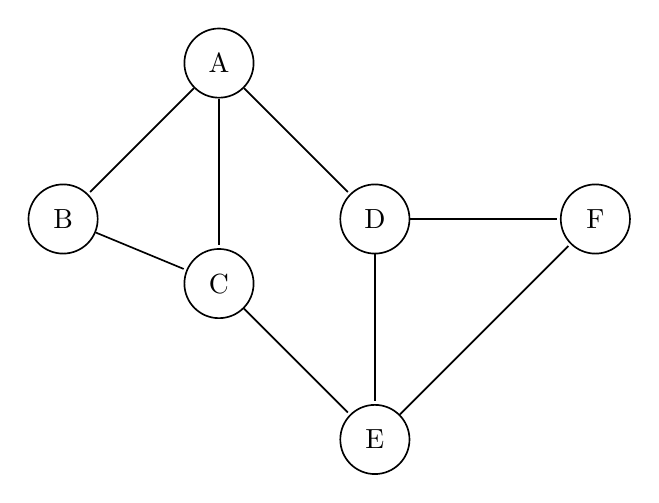
\begin{tikzpicture}[shorten >=1pt,auto,node distance=2.8cm,
                            semithick]

        \node[state]            (A)                         {A};
        \node[state]            (B) [below left of=A]       {B};
        \node[state]            (C) [below of=A]            {C};
        \node[state]            (D) [below right of=A]       {D};
        \node[state]            (E) [below of=D]            {E};
        \node[state]            (F) [right of=D]            {F};

        \path   (A) edge node {} (B)
                    edge node {} (C)
                    edge node {} (D)
                (B) edge node {} (C)
                (C) edge node {} (E)
                (D) edge node {} (E)
                    edge node {} (F)
                (E) edge node {} (F);

        \end{tikzpicture}

        \begin{enumerate}
            \item\label{DFT} With a depth-first traversal from A to F:

                \begin{answer}
                \begin{tabular}{|c|}
                ~\\
                ~\\
                A\\\hline
                \end{tabular}
                $\rightarrow$
                \begin{tabular}{|c|}
                B\\
                C\\
                D\\\hline
                \end{tabular}
                $\rightarrow$
                \begin{tabular}{|c|}
                ~\\
                C\\
                D\\\hline
                \end{tabular}
                $\rightarrow$
                \begin{tabular}{|c|}
                ~\\
                E\\
                D\\\hline
                \end{tabular}
                $\rightarrow$
                \begin{tabular}{|c|}
                ~\\
                ~\\
                D\\\hline
                \end{tabular}
                $\rightarrow$
                \begin{tabular}{|c|}
                ~\\
                ~\\
                F\\\hline
                \end{tabular}
                Path: A $\rightarrow$ B $\rightarrow$ C $\rightarrow$ E
                $\rightarrow$ D $\rightarrow$ F.
                \end{answer}

            \item With a breadth-first traversal from A to F:

                \begin{answer}
                \begin{tabular}{c}
                \hline
                A\\\hline
                \end{tabular}
                $\rightarrow$
                \begin{tabular}{c}
                \hline
                BCD\\\hline
                \end{tabular}
                $\rightarrow$
                \begin{tabular}{c}
                \hline
                CD\\\hline
                \end{tabular}
                $\rightarrow$
                \begin{tabular}{c}
                \hline
                DE\\\hline
                \end{tabular}

                Path: A $\rightarrow$ D $\rightarrow$ F.
                \end{answer}

        \end{enumerate}

    \item When we traverse a graph, either depth-first or breadth-first, how do
        we keep track of the path to the goal state? That is, once we find a
        node, how do we find out what the path we took to get to it was?

        \begin{answer}
        We often use a dictionary that maps a node to the node that we came
        from to get to it. So, for \ref{DFT}, we would end up with a table like:
        \begin{tabular}{r|l}
        node & parent\\\hline
        F & D\\
        D & E\\
        C & A\\
        A & {\tt None}
        \end{tabular}

        To find the answer, we just follow each node to its parent until we
        reach {\tt None}.
        \end{answer}

\section*{Backtracking}
    \item The algorithm below is broken. Fix it.
    \begin{lstlisting}
        def solve(config):
          if not isGoal(config):
             return config
          else:
             for child in successors(config):
                solution = solve(child)
                if solution == None:
                   return solution
                return None
    \end{lstlisting}        
    \begin{answer}
    \begin{lstlisting}
        def solve(config):
          """solve: Config -> Config or NoneType"""
          if isGoal(config):
             return config
          else:
             for child in successors(config):
                if isValid(child):
                    solution = solve(child)
                    if solution != None:
                       return solution
             return None
    \end{lstlisting}
    \end{answer}
    
    \item
    \begin {enumerate}
        \item What functions need to be written for your corrected code above to run? 
            \begin{answer}
                \begin{enumerate}
                  \item isGoal( config )
                  \item sucessors( config )
                  \item isValid( config )
                \end{enumerate}
            \end{answer}
        \item What must these functions return?
            \begin{answer}
                \begin{enumerate}
                    \item isGoal( config ) returns a bool
                    \item successors( config ) returns a list of possible successor configurations
                    \item isvalid( config ) returns a bool
                \end{enumerate}
            \end{answer}
    \end{enumerate}

\pagebreak
\section*{Djkstra's}  
    \item Perform Dijkstra's shortest path algorithm on the following
    weighted graph to find the shortest path between A and D. Show the
    order vertices are finalized. What is the cost from A to D? \\

\begin{centering}
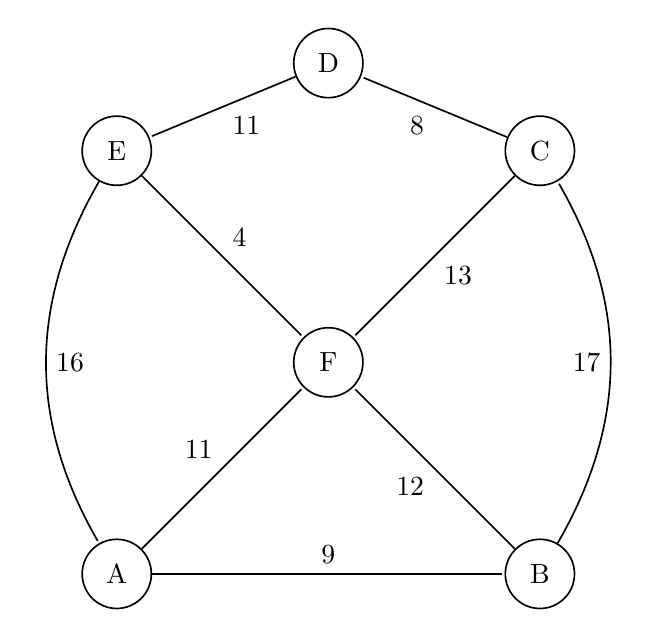
\begin{tikzpicture}[shorten >=1pt,auto,node distance=3.8cm,
                    semithick]
      \node[state](F)                    {F};
      \node[state](A) [below left  of=F] {A};
      \node[state](B) [below right of=F] {B};
      \node[state](C) [above right of=F] {C};
      \node[state](D) [above       of=F] {D};
      \node[state](E) [above left  of=F] {E};
      \path (A) edge                  node {9}  (B)
            (B) edge [bend right]     node {17} (C)
            (C) edge                  node {8}  (D)
            (D) edge                  node {11} (E)
            (E) edge [bend right]     node {16} (A)
            (A) edge                  node {11} (F)
            (B) edge                  node {12} (F)
            (C) edge                  node {13} (F)
            (E) edge                  node {4}  (F);
 \end{tikzpicture} \\
 \end{centering}
 \begin{answer}    
    Finalized order: A B F E C D \\
    Path: A F E D \\
    Cost: 26 \\
 \end{answer}

\end{enumerate}

\end{document}
